
%% cross-references, and citations.

\documentclass[11pt]{book}
\usepackage{Wiley-AuthoringTemplate}
\usepackage[sectionbib,authoryear]{natbib}
% for name-date citation comment the below line
%\usepackage[sectionbib,numbers]{natbib}% for numbered citation comment the above line

%%********************************************************************%%
%%       How many levels of section head would you like numbered?     %%
%% 0= no section numbers, 1= section, 2= subsection, 3= subsubsection %%
\setcounter{secnumdepth}{3}
%%********************************************************************%%
%%**********************************************************************%%
%%     How many levels of section head would you like to appear in the  %%
%%				Table of Contents?			%%
%% 0= chapter, 1= section, 2= subsection, 3= subsubsection titles.	%%
\setcounter{tocdepth}{2}
%%**********************************************************************%%

%\includeonly{ch01}
\makeindex
\usepackage{pdfpages}
\usepackage{hyperref}
\newcommand\Emph{\textbf}
\newcommand\p{^{\prime}}
\newcommand\pp{^{\prime\prime}}
\newcommand{\lapl}[1]{\mathscr{L}\{#1\}}
\newcommand{\X}{\mathbb{X}}
\newcommand{\dX}{\dot{\mathbb{X}}}
\newcommand{\fX}{\bar{\text{\b{X}}}}
\newcommand{\ux}{u_x}
\newcommand{\uy}{u_y}
\newcommand{\uxx}{u_{xx}}
\newcommand{\uxy}{u_{xy}}
\newcommand{\uyy}{u_{yy}}
\newcommand{\second}{2^{\text{nd}}}
\newcommand{\deriv}[2]{\frac{\diff#1}{\diff#2}}
\newcommand{\deriva}[1]{\frac{\diff}{\diff#1}}
\newcommand{\dakuohao}[2]{\left\{\begin{gathered}#1\\#2\end{gathered}\right.}
%\includeonly{week10/Wednesday}

\begin{document}

\frontmatter


\booktitle{Partial differential equations}

\subtitle{MAT4022 Notebook}

\AuAff{Prof. Weiming Ni\\ The Chinese University of Hongkong, Shenzhen}


\halftitlepage
\titlepage



\tableofcontents


\acknowledgments
This book is from the MAT4022 in fall semester, 2019. In addition, some material is cited from {\it Partial Differential Equations} $4^{th}$ edition by F.John.
\authorinitials{CUHK(SZ)}


\mainmatter
\setcounter{page}{1}


\chapter{Week1}

\section{Tuesday}\index{Tuesday_lecture}
\subsection{Introduction and Examples}
$u(x,y)$ a smooth function\\
$u_x=\frac{\partial u}{\partial x}$\\
$u_y=\frac{\partial u}{\partial y}$\\
$u_{xx}=\frac{\partial ^2u}{\partial x\partial x}$\\
$u_{xy}=\frac{\partial ^2u}{\partial y\partial x}$\\
In this course, as $u$ is smooth, we don't fuss about difference between $u_{xy}$ and $u_{yx}$.\\
\begin{definition}
A PDE is a relation for $F(x,y,u,u_x,y_y,u_{xy},\dots)=0$
linear equation.  If $F$ is linear in $u$, $u_x$, $u_y$, $u_{xx}$, $\cdots$ (Not necessarily in $x$, $y$)
\end{definition}

\begin{example}
Laplace equation: $u_{xx} + u_{xy} = 0$\\
$( x^2 + y^2 ) u_{xx} + e^{xy} u_{yy} = 0$\\
In the second case, it is still linear as it is a linear equation for $u_{xx}$ and $u_{yy}$. 
\end{example}
Other examples\\
Cauchy-Riemann.\\

$\begin{cases}
u_x - v_y = 0 \\
u_y + v_x = 0
\end{cases}$ 1st order system\\
$\begin{cases}u_{xx}-v_{yx}=0\\u_{yy}+v_{yx}\end{cases}\rightarrow u_{xx}+y_{yy}=0$ harmonic function ($2^{\text{st}}$ order).\\
Order: highest order that partial derivatives are taken.\\
Notation for laplace operator:
\[\Delta u=u_{xx}+u_{yy},~ \Delta u=u_{xx},~ \Delta u=u_{x_1x_1}+\cdots +u_{x_nx_n}\]
\begin{example}
Wave equation. $u_{tt}=c^2\Delta u$, $c>0$ wave speed a constant, $t$: time.\\
$n=1$ $u_tt=c^2u_{xx}$: vibration of a string\\
$n=2$ $u_{tt}=c^2(u_{xx}+u_{yy})$: water wave\\
$n=3$ $u_{tt}=c^2(u_{x_1x_1}+u_{x_2x_2}+u_{x_3x_3})$: sound wave\\
n: space dimension\\
n=1 A string, flexible, elastic, homogeneous with density $\rho$
\begin{figure}[H]
\centering
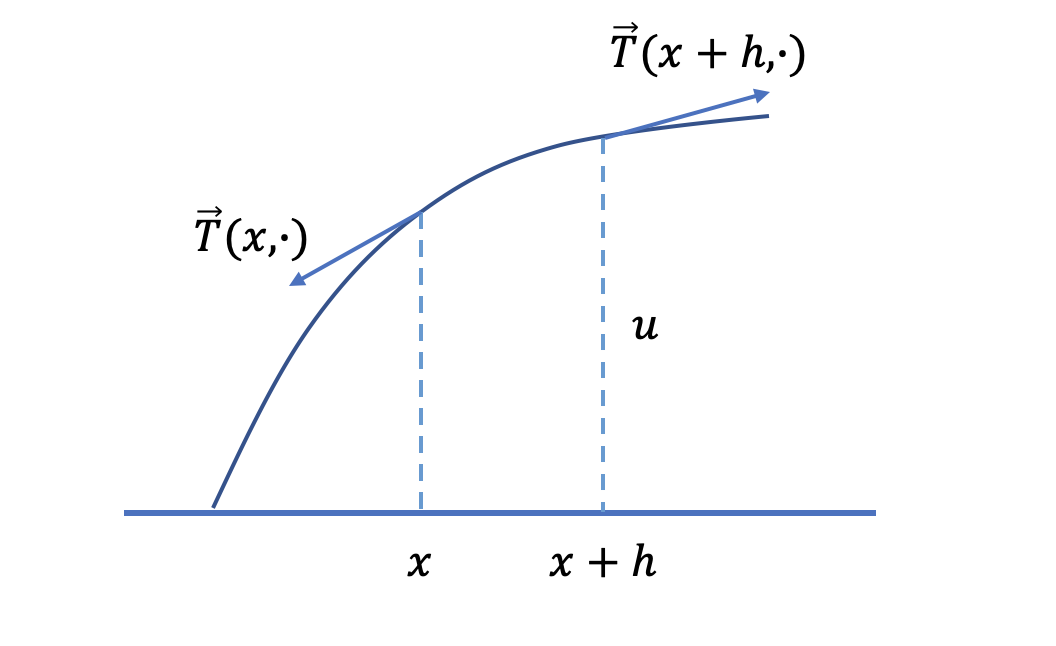
\includegraphics[width=10cm]{week1_tuesday1}
\end{figure}
\begin{figure}[H]
\centering
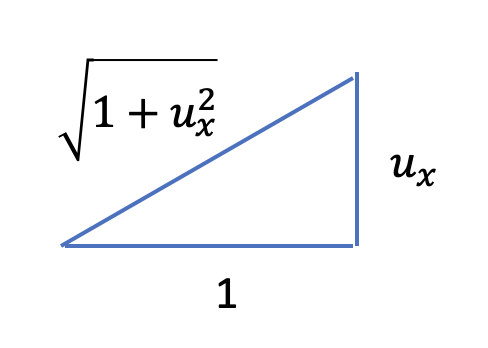
\includegraphics[width=6cm]{week1_tuesday2}
\end{figure}
When we magnefy part of the string and let $h$ to be small enough. The horizontal parts of  forces of $\vec{T}(x,\cdot)$ and $\vec{T}(x+h,\cdot)$ are equal to each other. Vertical forces is equal to $am$ according to Newton's second law. Therefore, we have the following.
\[\left\{\begin{gathered}\frac{|T|(x+h,\cdot)}{\sqrt{1+u_x^2(x+h,\cdot)}}=\frac{|T|(x,\cdot)}{\sqrt{1+u_x^2(x,\cdot)}}\\\frac{|T|u_x}{\sqrt{1+u_x^2}}(x+h,\cdot)-\frac{|T|u_x}{\sqrt{1+u_x^2}}(x,\cdot)=h\rho u_{tt}\end{gathered}\right.
\]
When $h$ is small enough,
\[\frac{1}{\sqrt{1+u_x^2}}=(1+u_x^2)^{-\frac{1}{2}}=1-\frac{1}{2}u_x^2+\cdots\approx1
\]
\[|T|(x+h,\cdot)=|T|(x,\cdot)
\]
\[\rho u_{tt}=|T|\cdot[u_x(x+h,\cdot)-u_x(x,\cdot)]\frac{1}{h}\rightarrow |T|u_{xx}
\]
\[u_{tt}=\frac{|T|}{\rho}u_{xx},~ c=\sqrt{\frac{|T|}{\rho}}
\]

\end{example}
\begin{example}[Heat equation]
$u_t=\Delta u$, u: temprature\\
$\begin{aligned}H(t)&=\text{total amount of heat in } \Omega\subset\mathbb{R}^3\\
&=\underset{\Omega}{\int\int\int}c\rho u \diff x\diff y\diff z
\end{aligned}$
\[\underset{\partial\Omega}{\int\int}\kappa\vartriangle u \nu\diff s=\frac{\diff H}{\diff t}=\underset{\Omega}{\int\int\int}c\rho u \diff x\diff y\diff z
\]
$\kappa$ is heat conduction constant. $\nu$ is unit outward normal.\\
\[\vec{w}=\vartriangle u=(u_x,u_y,u_z)
\]
\[\text{dir} \vec{w}=u_{xx}+u_{yy}+u_{zz}=\Delta u
\]
By divergent theorem:
\[\underset{\Omega}{\int\int\int}c\rho u_t=\underset{\Omega}{\int\int\int}\kappa\Delta u
\]
As this is the case for all $\Omega$ we can tell $c\rho u_t=\kappa\Delta u$
\[u_t=\frac{\kappa}{c\rho}{\Delta u}
\]
\end{example}
\begin{theorem}[Divergent theorem]
$\vec{w}=(w_1,w_2,w_3)$: vector field\\
\[\underset{\Omega}{\int\int\int}\text{dir}\vec{w}\diff x\diff y\diff z=\underset{\partial\Omega}{\int\int}\vec{w}\nu\diff s
\]
where $\text{dir}\vec{w}=\frac{\partial w_1}{\partial x}+\frac{\partial w_2}{\partial y}+\frac{\partial w_3}{\partial z}$




\end{theorem}









\section{Thursday}\index{Thursday_lecture}
\subsection{Examples}
Minimal surface equation.\\
Given a curve $\Gamma$ in $\mathbb{R}^3$ to find a surface spanning $\Gamma$ and has the smallest possible area.
\[(1+u_y^2)u_{xx}-2u_xu_yu_{xy}+(1+u_x^2)u_{yy}=0
\]
This is a $\second$ order linear in $\uxx,\uyy$ equation. It is called quasi-linear equation.\\
Now, before we take a look at solving some partial differential equations. Let's review a simple ode case.\\
In ODE,
\[v\p+cv=0
\]
\[\frac{\diff v}{\diff t}=v\p=-cv
\]
\[\frac{\diff v}{v}=-c\diff t
\]
At the moment, just ignore $|v|$
\[\ln v=-ct+\alpha
\]
\[v(t)=e^{-ct}e^\alpha=v(0)e^{-ct}, t=0~ v(0)=e^\alpha
\]
In PDE,
\[\uy+c\ux=0 ~c\text{: constant}
\]
This is called transport equation. Later on, we will talk about this name.
\[\deriva{t}u(x(t),y(t))=u_x\deriv{x}{t}+\uy\deriv{y}{t}=c\ux+\uy=0
\]
\[\left\{\begin{gathered}\deriv{x}{t}=c\\\deriv{y}{t}=1\end{gathered}\right.~\Rightarrow~\left\{\begin{gathered}x=ct+X(0)=ct+\xi\\y=t+y(0)=t\end{gathered}\right.
\]
\[\Rightarrow \xi=x-ct\qquad\xi=x-cy\]
On $\Gamma_\xi$, $\deriv{t}u(x(t),y(t))\equiv0$ $\forall t \Rightarrow$, $u(x(t),y(t))\equiv$ constant on $\Gamma_\xi$.\\
\[u(x,y)=f(x-cy)
\]
As convention, let $t$ denote $y$, transport equation is $\begin{cases}u_t+c\ux=0\\u(x,0)=f(x)\end{cases}~\Rightarrow~u(x,t)=f(x-ct)$.\\
The following is a graph used to illustrate why it is called transport equation:
\[u(cT,T)=f(cT-cT)=f(0)=u(0,0)
\]
\begin{figure}[H]
\centering
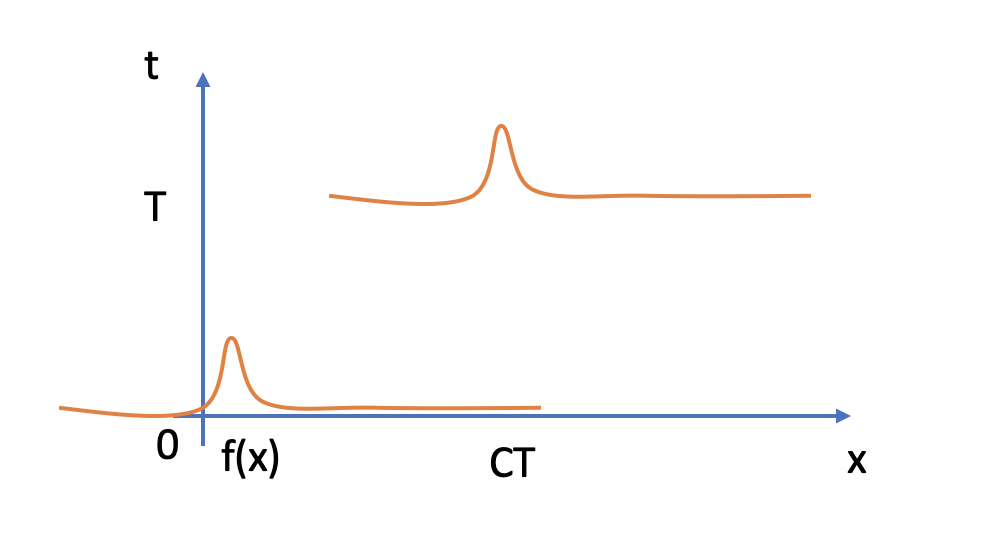
\includegraphics[width=10cm]{week1_thursday1}
\end{figure}
\begin{example}
\[\left \{\begin{gathered}x\ux+y\uy=\alpha u\\u(x,1)=f(x)\end{gathered}\right.
\]
$\Gamma:$ characteristic curve $\dakuohao{\deriv{x}{t}=x}{\deriv{y}{t}=y}~\Rightarrow~\dakuohao{x=x_0e^t=se^t}{y=y_0e^t=1e^t~\rightarrow~t=\ln y}$.\\
Initial curve $\dakuohao{x=s}{y=1}$.\\
\[s=\frac{x}{e^t}=\frac{x}{y}
\]
On $\Gamma$, we have $\deriv{u}{t}=\ux\deriv{x}{t}+\uy\deriv{y}{t}=x\ux+y\uy=\alpha u\Rightarrow u=ce^{\alpha t}=f(s)e^{\alpha}$
About the last equal sign of above equation, it is because $u(x_0,y_0)=u(s,1)=c$ when t=0.
\[u(x,y)=f(\frac{x}{y})y^\alpha
\]


\end{example}
Next lecture will discuss quasi-linear equation.
\[a(x,y,u)\ux+b(x,y,u)\uy=c(x,y,u)
\]



\chapter{week2}

\section{Tuesday}\index{Tuesday_lecture}
\subsection{Quasi-linear Equations}
Review: last week we have learn how to solve the following PDE and get the solution along characteristic curves.
\[\uy+c\ux=0\qquad x\ux+y\uy=u
\]
\begin{figure}[H]
\centering
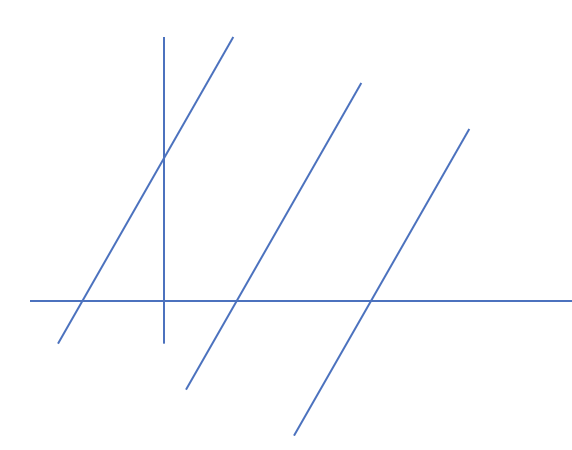
\includegraphics[width=3cm]{week2_tuesday1}
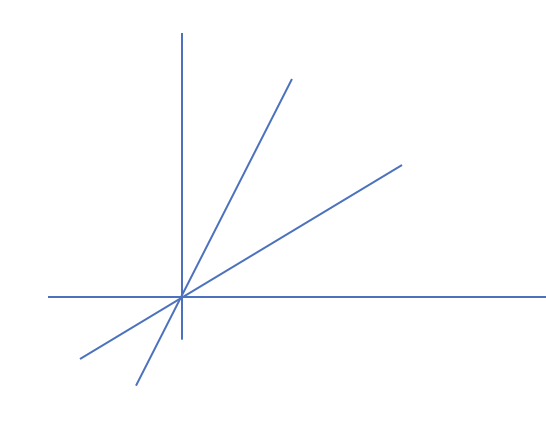
\includegraphics[width=3cm]{week2_tuesday2}
\end{figure}
\[a(x,y,u)\ux+b(x,y,u)\uy=c(x,y,u)
\]
This is what we called quasi-linear equation. At this time, I have to quote our textbook p9 since I cannot explain what professor said better than it does.
\begin{figure}[H]
\centering
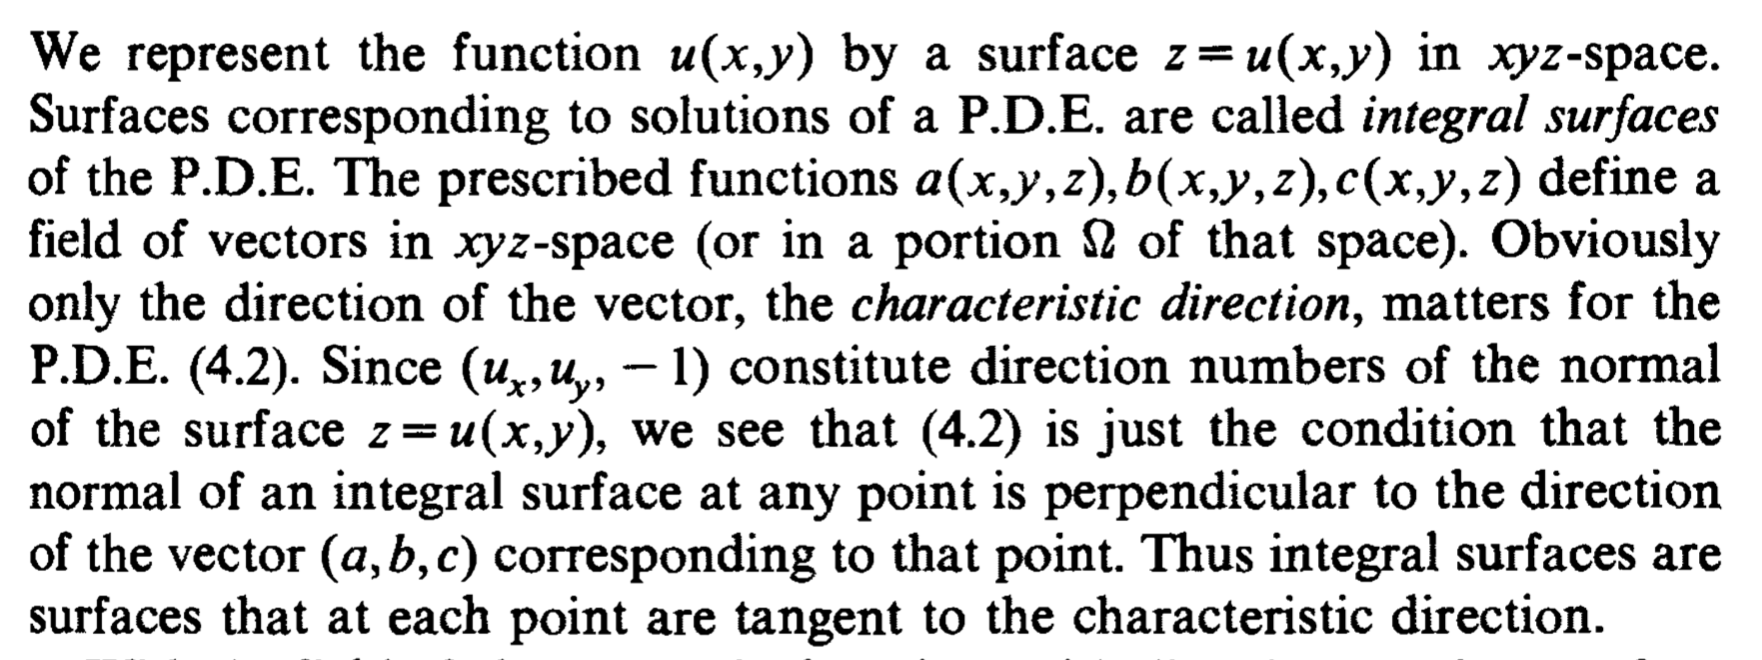
\includegraphics[width=15cm]{week2_tuesday3}
\end{figure}
\begin{figure}[H]
\centering
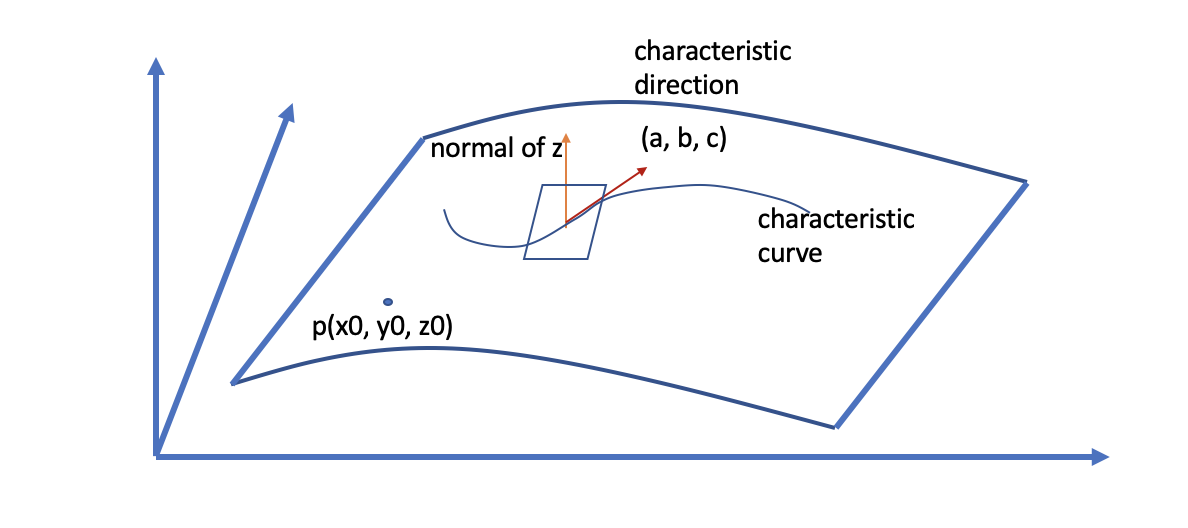
\includegraphics[width=15cm]{week2_tuesday4}
\end{figure}
Next we are going to show that the integral surface, that is the solution $u$ we want, is the union of characteristic curves.
\begin{theorem}
If a characteristic curve $\mathscr{C}$ has one point on a integral surface $z=u(x,y)$ then $\mathscr{C}$ lies entirely on the surface.

\end{theorem}
\begin{proof}
\[z_0=u(x_0,y_0)
\]
\[\left\{\begin{gathered}\deriv{x}{t}=a(x(t),y(t),u(x_0,y_0))\\\deriv{y}{t}=b(x(t),y(t),u(x_0,y_0))\\x(0)=x_0\\y(0)=y_0\end{gathered}\right.
\]
This is a system of odes, there is a solution ($x(t),y(t)$) when $t$ is around 0.\\
This gives us a curve $(x(t),y(t),u(x(t),y(t)))$ lies on the integral surface.\\
Claim: It's a characteristic curve.
\[z(t)=u(x(t),y(t))
\]
\[\deriv{z}{t}=\ux\deriv{x}{t}+\uy\deriv{y}{t}=a\ux+b\uy=c
\]



\end{proof}
\subsection{Cauchy Problem}
``Finding the function $u(x,y)$ for given data $f(s)$, $g(s)$, $h(s)$ constitutes the \text{\it Cauchy problem} for quasi-linear equation.'' (John, 1982, p.9)\\ The following $\varphi, \psi, \rho$ are $f, g, h$ correspondingly.\\
To solve the Cauchy problem, it suffices to require that $(\psi\p,\varphi\p)\&(a,b)$ are linearly independent.\\The
\[\left\{\begin{gathered}\deriv{\bar{X}}{t}=a(\bar{X},\bar{Y},Z)\\\deriv{\bar{Y}}{t}=b(\bar{X},\bar{Y},Z)\\\deriv{\bar{z}}{t}=c(\bar{X},\bar{Y},Z)\\\bar{X}(s,0)=\varphi(s)\\\bar{Y}(s,0)=\psi(s)\\\bar{Z}(s,0)=\rho(s)\end{gathered}\right.
\]
Existence and uniqueness theorem for ODE.\\
$\Rightarrow$ For every $s$, $\exists$ one solution $(\bar{X}(s,t),\bar{Y}(s,t),z(s,t))$. In order to make $u(x,y)=z(s(x,y),t(x,y))$ is the case. We need implicit function theorem which makes us able to write $s, t$ as a function of $(x,y)$
\[\begin{vmatrix}\frac{\partial{\bar{X}}}{\partial{s}}&\frac{\partial{\bar{X}}}{\partial{t}}\\\frac{\partial{\bar{Y}}}{\partial{s}}&\frac{\partial{\bar{Y}}}{\partial{t}}\end{vmatrix}=\begin{vmatrix}\varphi\p&a\\\psi\p&b\end{vmatrix}\neq0
\]
\begin{example}
\[\uy+u\ux=0, \quad u(x,0)=f(x)\]
\[\deriv{x}{t}=z,~\deriv{y}{t}=1,~\deriv{z}{t}=0
\]
$z$ is constant in $t$. $z(s, 0)=f(s)\Rightarrow z(s,t)=f(s)$.
\[\dakuohao{x(s,0)=s~\Rightarrow~x(s,t)=f(s)t+s}{y(s,0)=0~\Rightarrow~y(s,t)=t}\rightarrow ~s=x-f(s)t=x-f(s)y=x-zy
\]
\[z(s,0)=f(s)\Rightarrow z(s,t)=f(s)=f(x-zy)
\]
\[u(x,y)=f(x-uy)
\]
Characteristic curve
\[f(s_2)>f(s_3)
\]
\[\frac{1}{f(s_2)}<\frac{1}{s_3}
\]
Why it is called a ``Shock''?\\The reason is that: for same $(x,y)$ $z$ should be the same. However, from the graph we can see there are two $z$ corresponds to the same point marked by the circle. Therefore, the solution does't exist.
\begin{figure}[H]
\centering
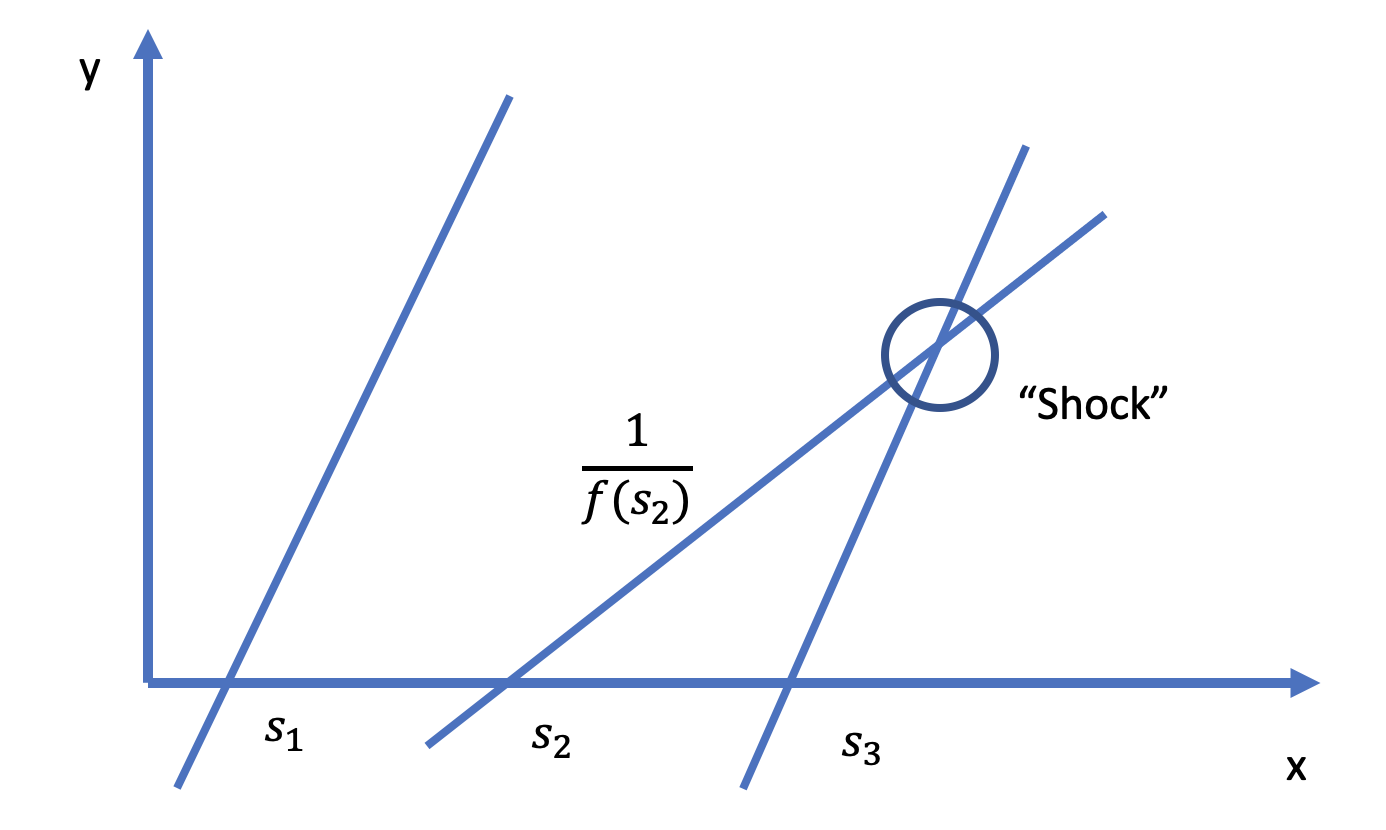
\includegraphics[width=8cm]{week2_tuesday5}
\end{figure}



\end{example}

\section{Thursday}\index{Thursday_lecture}
\subsection{$\second$ order Quasi-linear}
\[a\uxx+2b\uxy+c\uyy=d
\]
$a$, $b$, $c$, $d$ are functions of $(x,y,u,\ux,\uy)$\\
Initial curve $f(s)$, $g(s)$. Initial value $u=h(s),\ux=\varphi(s), \uy=\psi(s)$.\\
\[u(f(s),g(s))=h(s)
\]
\[\ux f\p+\uy g\p=h\p
\]
\[\varphi f\p+\psi g\p=h\p
\]
Assume the above equation is satisfied.
\[\ux(f(s),g(s))=\varphi(s)\qquad\uy(f(s),g(s))=\psi(s)
\]
\[\uxx f\p+\uxy g\p=\varphi \p\qquad u_{yx}f\p+\uyy g\p=\psi\p
\]
\[\begin{pmatrix}a&2b&c\\f\p&g\p&0\\0&f\p&g\p\end{pmatrix}\begin{pmatrix}\uxx\\\uxy\\\uyy\end{pmatrix}=\begin{pmatrix}d\\\varphi\p\\\psi\p\end{pmatrix}
\]
\[0=\begin{vmatrix}a&2b&c\\f\p&g\p&0\\0&f\p&g\p\end{vmatrix}=a{g\p}^2-2bf\p g\p+c{f\p}^2
\]
Personal understanding (may not be correct):\\
This is called characteristic curve for when determinant is equal to zero above system will not have a solution. This situation will on happen when the initial curve $(f,g,h)$is tangent to a charateristic curve at every point. Therefore, $a{g\p}^2-2bf\p g\p+c{f\p}^2$.
\[\dakuohao{x=f(s)}{y=g(s)}\quad\dakuohao{\deriv{x}{s}=f\p}{\deriv{y}{s}=g\p}~\Rightarrow~\deriv{y}{x}=\frac{g\p}{f\p}
\]
\[a(\deriv{y}{x})^2-2b\deriv{y}{x}+c=0
\]
\[\deriv{y}{x}=\frac{2b\pm\sqrt{2b^2-4ac}}{2a}
\]
\begin{itemize}
\item $b^2-ac>0$: Hyperbolic
\item $b^2-ac=0$: Parabolic
\item $b^2-ac<0$: Elliptic

\end{itemize}
\begin{example}

\begin{itemize}
\item $\uyy-c^2\uxx=0$ $A=-c^2, B=0, C=1\Rightarrow~B^2-AC=C^2$
\item heat equation $\uy=c^2=\uxx=0$  $A=-C^2, B=0, C=0~\Rightarrow~B^2-AC=0$
\item laplace equation $\uyy+\uxx=0$ $A=1=C, B=0~\Rightarrow~B^2-AC=-1<0$
\end{itemize}
\end{example}

Wave equation
\[\uyy-c^2\uxx=0
\]
\[\deriv{y}{x}=\frac{1}{-c^2}(\pm c)=\mp\frac{1}{c}
\]
\[y=\mp\frac{1}{c}x+\text{const}
\]
\[y\pm\frac{1}{c}x=\text{const}
\]
\[\xi=y+\frac{1}{c}x
\]
\[\eta=y-\frac{1}{c}x
\]
\[v(\xi,\eta)=u(x(\xi,\eta),y(\xi,\eta))
\]
\[u(x,y)=v(\xi(x,y),\eta(x,y))
\]
\[\ux=v_{\xi}\xi_{x}+v_\eta\eta_x=v_{\xi}\frac{1}{c}-v_\eta\frac{1}{c}
\]
\[\uxx=v_{\xi\xi}\frac{1}{c^2}+v_{\xi\eta}(-\frac{1}{c^2})-v_{\eta\xi}\frac{1}{c^2}+v_{\eta\eta}\frac{1}{c^2}
\]
\[\uy=v_\xi\xi_y+v_\eta\eta_y=v_\xi+v_\eta
\]
\[\uyy=v_{\xi\xi}+2v_{\xi\eta}+v_{yy}
\]
\[0=\uyy-c^2\uxx=v_{\xi\xi}+2v_{\xi\eta}+v_{yy}-v_{\xi\xi}+2v_{\xi\eta}-v_{\eta\eta}=4v_{\xi\eta}
\]
\[v_{\eta\xi}=0~\Rightarrow~(v_\xi)_\eta=0~\Rightarrow ~v_\xi=f\p(\xi)
\]
\[v=f(\xi)=\text{const in }\xi
\]
\[v(\xi,\eta)=f(\xi)+g(\eta)=u(x,y)=f(y+\frac{1}{c}x)+g(y-\frac{1}{c}x)
\]
An observation:
\[u(A)+u(C)=f(y_A+\frac{1}{c}x_A)+g(\underline{\red y_A-\frac{1}{c}x_A})+f(y_C\frac{1}{c}x_C)+g(y_C-\frac{1}{c}x_C)
\]
\[u(B)+u(D)=f(y_B+\frac{1}{c}x_B)+g(\underline{\red y_B-\frac{1}{c}x_B})+f(y_D\frac{1}{c}x_D)+g(y_D-\frac{1}{c}x_D)
\]
\begin{figure}[H]
\centering
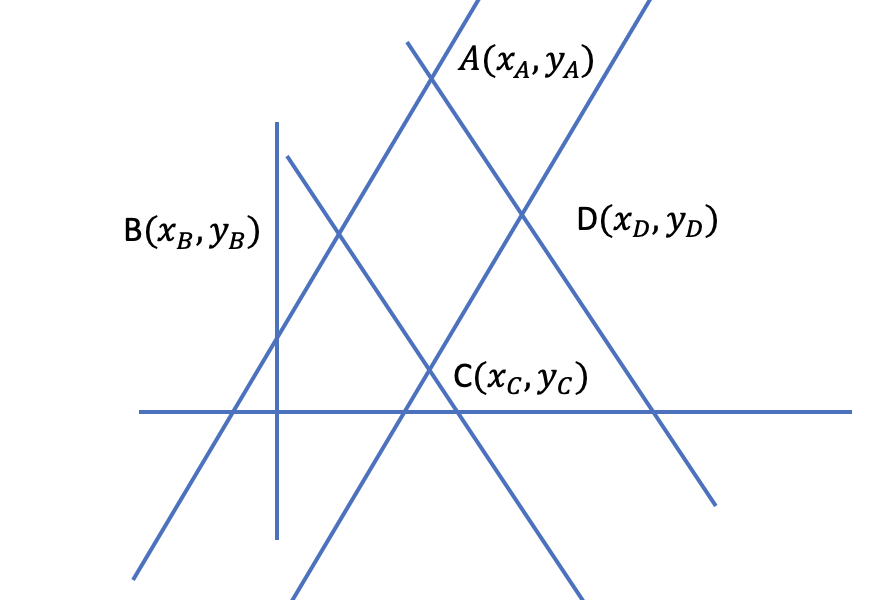
\includegraphics[width=8cm]{w2_th1}
\end{figure}
Take $c=1$ for simplicity
\[\left\{\begin{gathered}\uyy-\uxx=0\\u(x,0)=\varphi(x)\\\uy(x,0)=\psi(x)\end{gathered}\right.
\]
\[u(x,y)=f(y+x)+g(y-x)
\]
\[\varphi(x)=u(x,0)=f(x)+g(-x)
\]
\[\psi(x)=\uy(x,0)=f\p(x)+g\p(-x)
\]
\[\varphi(x)=f(x)+g(-x)~\Rightarrow~\varphi\p(x)=f\p(x)-g\p(-x)
\]
\[\dakuohao{\varphi(x)=f(x)=g(-x)}{\psi(x)=f\p(x)=g\p(x)}\Rightarrow \psi\p(x)=f\p(x)-g\p(-x)
\]
\[\frac{\varphi\p(x)+\psi(x)}{2}=f\p(x)\Rightarrow~f(x)=\frac{1}{2}\psi(x)+\frac{1}{2}\int_0^x\psi(s)\diff s+\text{const}\alpha
\]
\[\frac{-\varphi\p(x)+\psi(x)}{2}=g\p(-x)~\Rightarrow~g(-x)=\frac{1}{2}\varphi(x)-\frac{1}{2}\int_0^x\psi(s)\diff s+\text{const}\beta
\]
\[\begin{aligned}u(x,y)&=f(x+y)+g(y-x)\\&=\frac{1}{2}\varphi(x+y)+\frac{1}{2}\int_0^{x+y}\psi(s)\diff s+\alpha+\frac{1}{2}\varphi(x-y)-\frac{1}{2}\int_0^{x-y}\psi(s)\diff s+\beta\\&=\frac{1}{2}[\varphi(x+y)+\varphi(x-y)]+\frac{1}{2}\int_{x-y}^{x+y}\psi(s)\diff s+\alpha+\beta\end{aligned}
\]
\\
\[u(x,y)=\frac{1}{2}[\varphi(x+y)+\varphi(x-y)]+\frac{1}{2}\int_{x-y}^{x+y}\psi(s)\diff s
\]
\[\begin{cases}\uyy-\uxx=0\\u(x,0)=\varphi(x)\text{--initial displacement}\\\uy(x,0)=\psi(x)\text{--initial velocity}\end{cases}
\]
case(i) $\psi\equiv0$ $t=y=1$ $u(x,1)=\frac{1}{2}\varphi(x+1)+\frac{1}{2}\varphi(x-1)$
\begin{figure}[H]
\centering
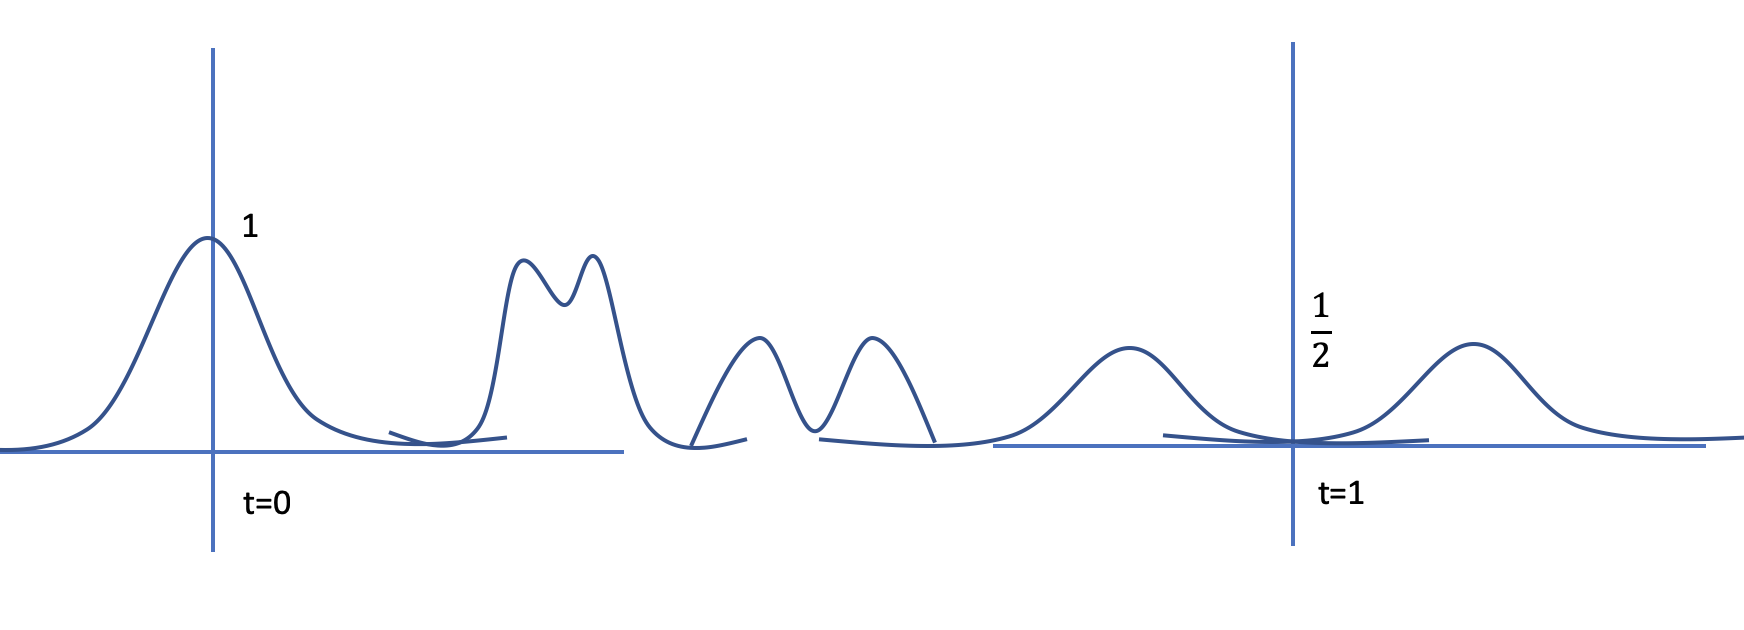
\includegraphics[width=12cm]{w2_th2}
\end{figure}
case(ii)$\psi=0$
\begin{figure}[H]
\centering
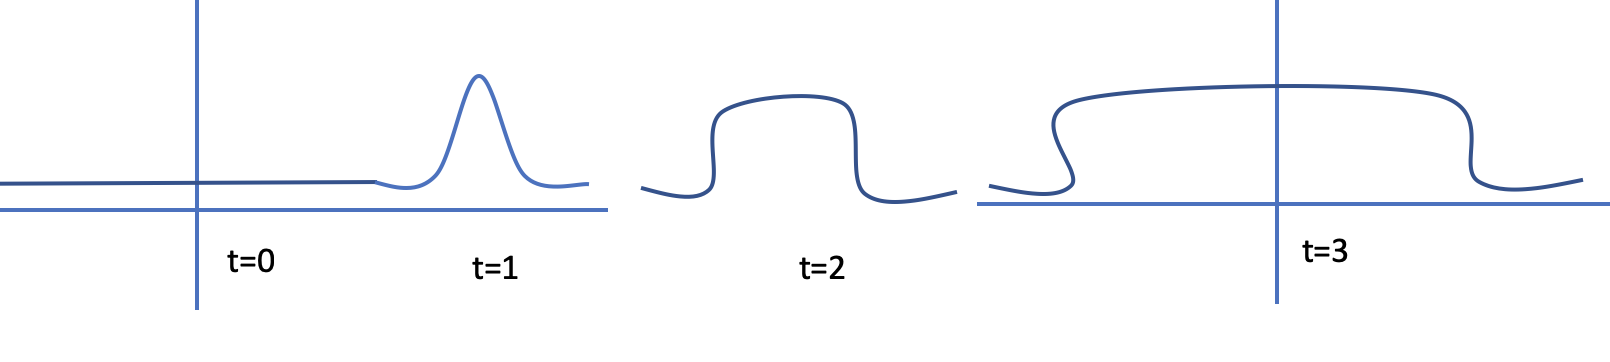
\includegraphics[width=13cm]{w2_th3}
\end{figure}
\chapter{week2}

\section{Tuesday}\index{Tuesday_lecture}
\subsection{Quasi-linear Equations}
Review: last week we have learn how to solve the following PDE and get the solution along characteristic curves.
\[\uy+c\ux=0\qquad x\ux+y\uy=u
\]
\begin{figure}[H]
\centering
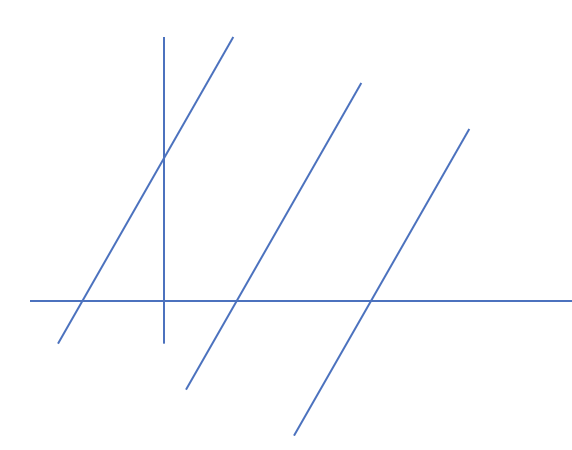
\includegraphics[width=3cm]{week2_tuesday1}
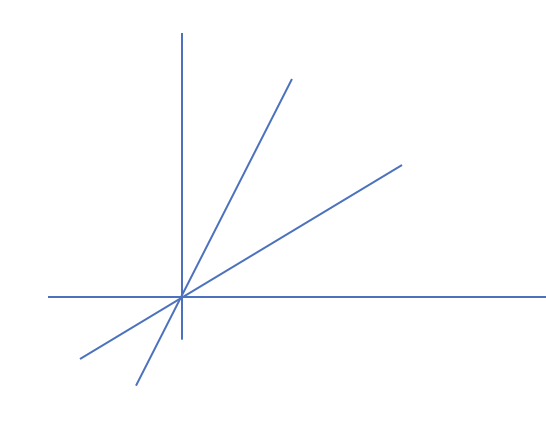
\includegraphics[width=3cm]{week2_tuesday2}
\end{figure}
\[a(x,y,u)\ux+b(x,y,u)\uy=c(x,y,u)
\]
This is what we called quasi-linear equation. At this time, I have to quote our textbook p9 since I cannot explain what professor said better than it does.
\begin{figure}[H]
\centering
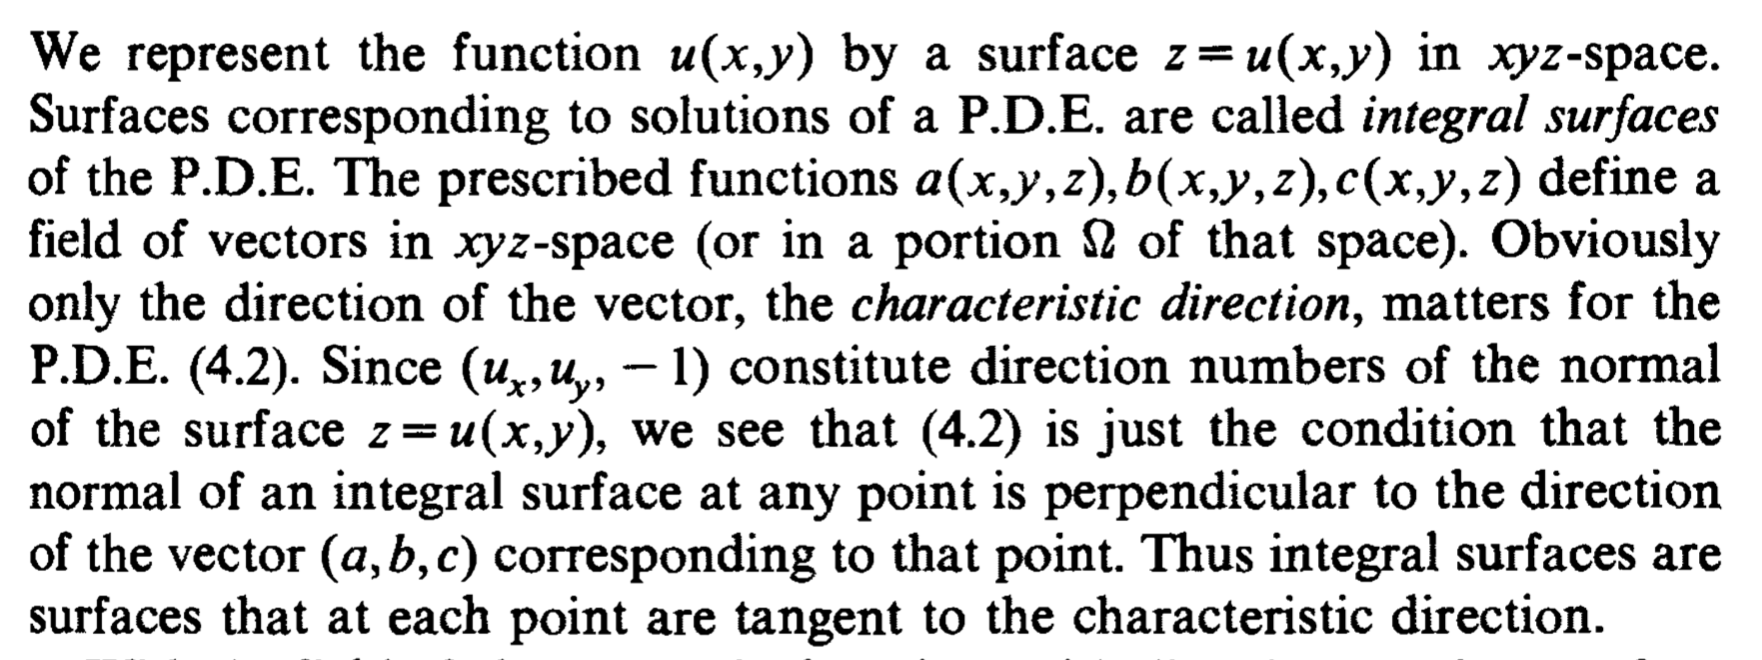
\includegraphics[width=15cm]{week2_tuesday3}
\end{figure}
\begin{figure}[H]
\centering
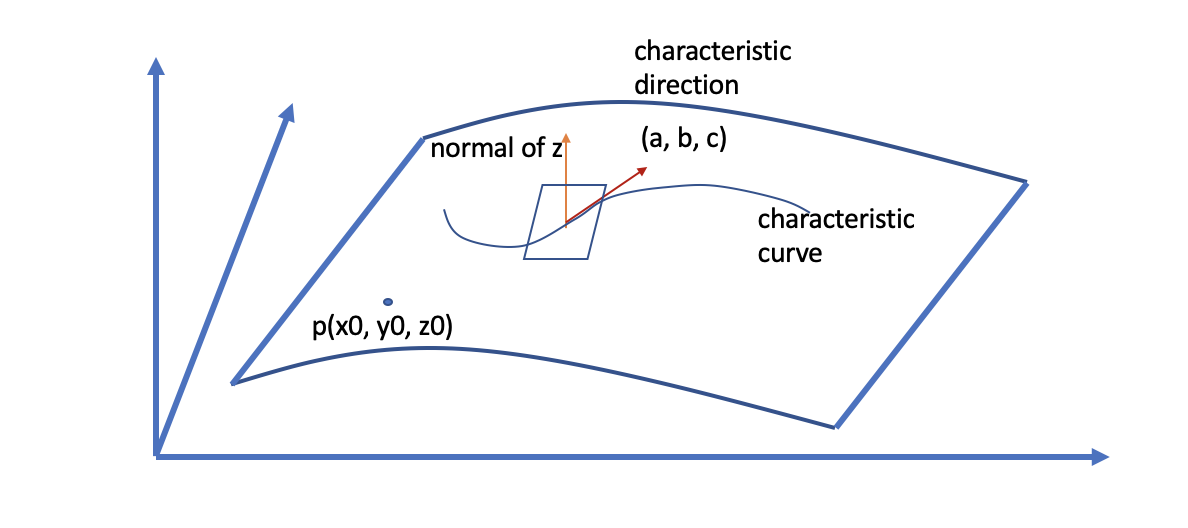
\includegraphics[width=15cm]{week2_tuesday4}
\end{figure}
Next we are going to show that the integral surface, that is the solution $u$ we want, is the union of characteristic curves.
\begin{theorem}
If a characteristic curve $\mathscr{C}$ has one point on a integral surface $z=u(x,y)$ then $\mathscr{C}$ lies entirely on the surface.

\end{theorem}
\begin{proof}
\[z_0=u(x_0,y_0)
\]
\[\left\{\begin{gathered}\deriv{x}{t}=a(x(t),y(t),u(x_0,y_0))\\\deriv{y}{t}=b(x(t),y(t),u(x_0,y_0))\\x(0)=x_0\\y(0)=y_0\end{gathered}\right.
\]
This is a system of odes, there is a solution ($x(t),y(t)$) when $t$ is around 0.\\
This gives us a curve $(x(t),y(t),u(x(t),y(t)))$ lies on the integral surface.\\
Claim: It's a characteristic curve.
\[z(t)=u(x(t),y(t))
\]
\[\deriv{z}{t}=\ux\deriv{x}{t}+\uy\deriv{y}{t}=a\ux+b\uy=c
\]



\end{proof}
\subsection{Cauchy Problem}
``Finding the function $u(x,y)$ for given data $f(s)$, $g(s)$, $h(s)$ constitutes the \text{\it Cauchy problem} for quasi-linear equation.'' (John, 1982, p.9)\\ The following $\varphi, \psi, \rho$ are $f, g, h$ correspondingly.\\
To solve the Cauchy problem, it suffices to require that $(\psi\p,\varphi\p)\&(a,b)$ are linearly independent.\\The
\[\left\{\begin{gathered}\deriv{\bar{X}}{t}=a(\bar{X},\bar{Y},Z)\\\deriv{\bar{Y}}{t}=b(\bar{X},\bar{Y},Z)\\\deriv{\bar{z}}{t}=c(\bar{X},\bar{Y},Z)\\\bar{X}(s,0)=\varphi(s)\\\bar{Y}(s,0)=\psi(s)\\\bar{Z}(s,0)=\rho(s)\end{gathered}\right.
\]
Existence and uniqueness theorem for ODE.\\
$\Rightarrow$ For every $s$, $\exists$ one solution $(\bar{X}(s,t),\bar{Y}(s,t),z(s,t))$. In order to make $u(x,y)=z(s(x,y),t(x,y))$ is the case. We need implicit function theorem which makes us able to write $s, t$ as a function of $(x,y)$
\[\begin{vmatrix}\frac{\partial{\bar{X}}}{\partial{s}}&\frac{\partial{\bar{X}}}{\partial{t}}\\\frac{\partial{\bar{Y}}}{\partial{s}}&\frac{\partial{\bar{Y}}}{\partial{t}}\end{vmatrix}=\begin{vmatrix}\varphi\p&a\\\psi\p&b\end{vmatrix}\neq0
\]
\begin{example}
\[\uy+u\ux=0, \quad u(x,0)=f(x)\]
\[\deriv{x}{t}=z,~\deriv{y}{t}=1,~\deriv{z}{t}=0
\]
$z$ is constant in $t$. $z(s, 0)=f(s)\Rightarrow z(s,t)=f(s)$.
\[\dakuohao{x(s,0)=s~\Rightarrow~x(s,t)=f(s)t+s}{y(s,0)=0~\Rightarrow~y(s,t)=t}\rightarrow ~s=x-f(s)t=x-f(s)y=x-zy
\]
\[z(s,0)=f(s)\Rightarrow z(s,t)=f(s)=f(x-zy)
\]
\[u(x,y)=f(x-uy)
\]
Characteristic curve
\[f(s_2)>f(s_3)
\]
\[\frac{1}{f(s_2)}<\frac{1}{s_3}
\]
Why it is called a ``Shock''?\\The reason is that: for same $(x,y)$ $z$ should be the same. However, from the graph we can see there are two $z$ corresponds to the same point marked by the circle. Therefore, the solution does't exist.
\begin{figure}[H]
\centering
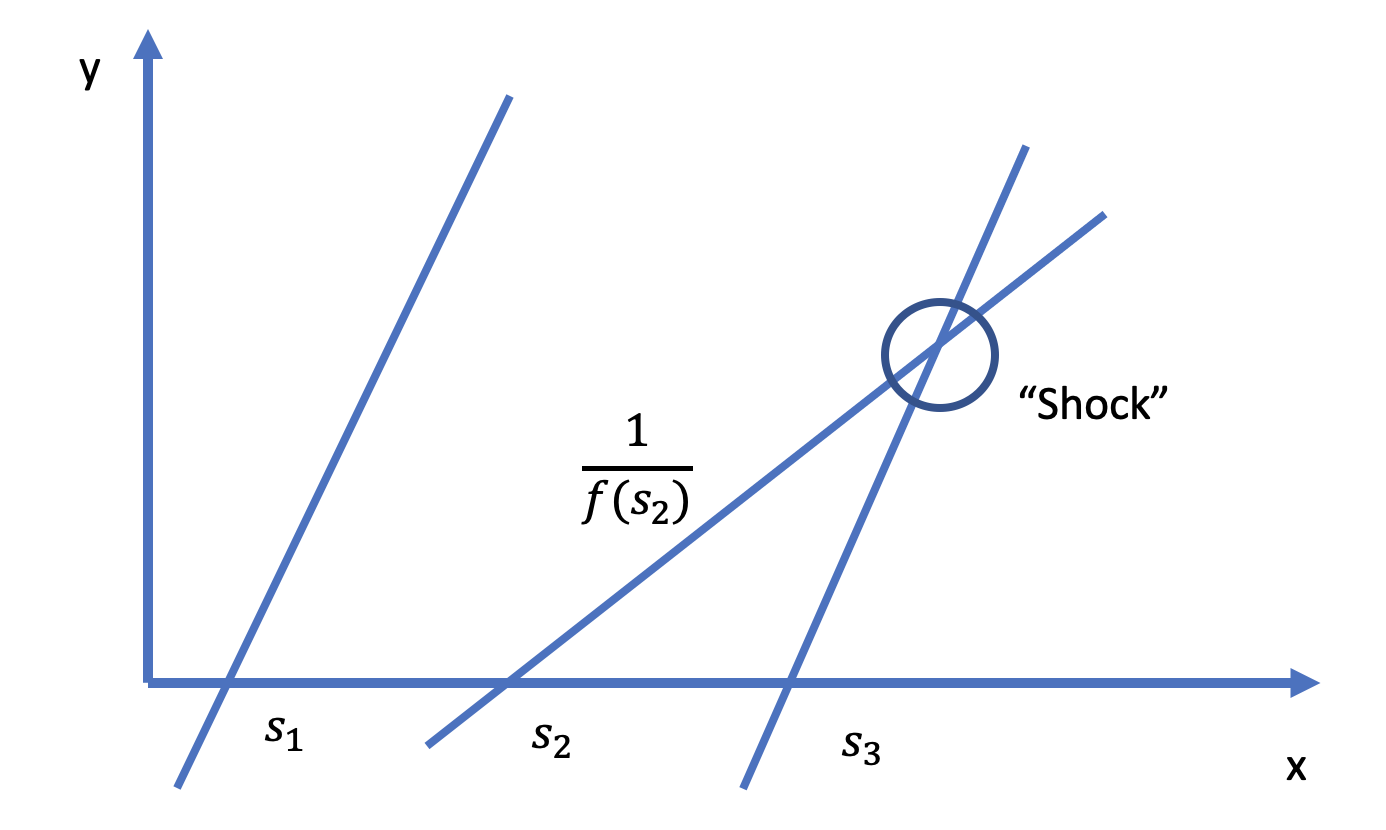
\includegraphics[width=8cm]{week2_tuesday5}
\end{figure}



\end{example}

\backmatter

\latexprintindex

\end{document}
